% ---
% Chapter 2
% ---
\chapter{Background}
\label{chapter:background}
% ---

Before jumping into the details of the implementation of \CSPcoq{}, we first need to understand some aspects of the CSP language itself, such as its syntax and semantics (Section~\ref{section:csp}). Beyond that, it is also important to provide an overview of the Coq proof assistant, covering concepts such as tactics, as well as the embedded Ltac language (Section~\ref{section:coq}). In this chapter, we also present the QuickChick property-based testing tool (Section~\ref{section:quickchick}), which is the Coq implementation of QuickCheck~\cite{hughes:quickcheck2000} -- a tool for testing properties randomly in Haskell.

% ---
\section{Communicating sequential processes}
\label{section:csp}
% ---

In 1978, Tony Hoare proposed a theory to help us understand concurrent systems, parallel programming and multiprocessing: \emph{Communicating Sequential Processes} \cite{hoare:csp}. More than that, it introduces a way to decide whether a concurrent program meets its specification. This theory quickly evolved into what is known today as the CSP specification language. This language belongs to a class of notations known as process algebras, where concepts of communication and interaction are presented in an algebraic style.

Since the main goal of CSP is to provide a theory-driven framework for designing systems of interacting components and reasoning about them, we must introduce the concept of a component, or as we will be referencing it from now on, a \emph{process}. Processes are self-contained entities that, once combined, can describe a system, which is yet another larger process that may itself be combined as well with other processes.

The way a process communicates with the environment is through its \emph{interface}. The interface of a process is the set of all the events that the process has the potential to engage in. An \emph{event} represents the atomic part of the communication. It is the piece of information the processes rely on to interact with one another. A process can either participate actively or passively in a communication, depending on whether it performed or suffered the consequences of an action. Events may be external, meaning they appear in the process interface; may indicate termination, represented by the event $ \tick $; or may be internal, and therefore unknown to the environment, denoted by the event $ \tau $.

One of the most basic process one can define is $ \mathit{\STOP} $. Essentially, this process never interacts with the environment and its only purpose is to denote the end of an execution without success, that is, in the sense of a failure or a \emph{deadlock}: a state in which the process can not engage in any event or make any progress whatsoever. It could be used to describe a computer that failed booting because one of its components is damaged, or a camera that can no longer take pictures due to storage space shortage.

Another basic process is $ \mathit{\SKIP} $. It indicates that the process has reached a successful termination state. We can use $ \mathit{\SKIP} $ to illustrate an athlete that has crossed the finish line, or a build for a project that has passed. But differently to $ \mathit{\STOP} $, $ \mathit{\SKIP} $ allows a continuation of behaviour when followed by a sequential composition operator, explained later on in this section.

Provided these two basic processes, $ \mathit{\STOP} $ and $ \mathit{\SKIP} $, and the knowledge of what the process interface is, we can apply a handful of CSP operators to define more descriptive processes. For example, let $ a $ be an event in the process $ P $ interface, one can define $ P $ as $ a \then \mathit{\STOP} $, meaning that this process behaves as $ \mathit{\STOP} $ after performing $ a $. In other words, the event $ a $ is offered to the environment and, as soon as this event is engaged by any actor in the system, the execution control is transferred immediately to the process $ \mathit{\STOP} $. This operator is known as the \emph{event prefix}, and it is pronounced as ``then''.

The choice between processes can be constructed in two different ways in CSP: externally and internally. To illustrate the difference between these choice operators, consider the following scenario: a cafeteria operates by letting the customers choose between ice cream and cake for desert. In this case, the choice is external to the business and it might be described using the \emph{external choice} operation: $ ice\_cream \then \mathit{\SKIP} \extchoice cake \then \mathit{\SKIP} $. An external choice between two processes implies the ability to perform any event that either sub-process can first engage in. Therefore, the environment has control over the outcome of such a decision.

Now, suppose that the cafeteria itself makes this choice (i.e. employees decide), having the clients no control over what deserts they will get. The decision would then become internal to the business, thus the \emph{internal choice} $ ice\_cream \then \mathit{\SKIP} \intchoice cake \then \mathit{\SKIP} $ would capture such a business rule. In an internal choice operation, the process itself is the only responsible for deciding which event from its interface will be communicated, therefore which sub-process it will resolve to. Note that this operation is essentially a source of non-deterministic behaviour.

CSP introduces two approaches for describing a parallel execution between processes: the \emph{alphabetised parallelism} and the \emph{generalised parallelism}. Let $ A $ be the interface of process $ P $, and $ B $ the interface of process $ Q $, an alphabetised parallel combination of these processes is described as $ P \parallel[A][B] Q $. Events in the intersection of $ A $ and $ B $ must be simultaneously engaged in by the processes $ P $ and $ Q $. In other words, an event that appears in both process interfaces can only be communicated if the two processes are ready to perform this event at the same moment. Any other event that does not match this criteria can be engaged in by its corresponding process independently.

The semantics is similar for the generalised version of the parallel operator. The only change is its constructor, which takes the synchronisation alphabet alone as the interface argument the processes must agree upon. Let $ C $ be the intersection of the previously defined interfaces $ A $ and $ B $, the generalised parallelism between processes $ P $ and $ Q $ is written as $ P \parallel[C] Q $.

Both versions of the parallel operator may be used to describe a marathon where every participant is a process that runs in parallel with each other. They must all start the race at the same time, but they are not expected to cross the finish line all together. We can use the alphabetised parallel operator to specify the combination between two participants as $ \mathit{RUNNER1} \parallel[\{start, finish1\}][\{start, finish2\}] \mathit{RUNNER2} $, or use the generalised version of the operator instead: $ \mathit{RUNNER1} \parallel[\{start\}] \mathit{RUNNER2} $.

Another CSP operator that models concurrent execution of processes is the \emph{interleaving} one. Different from the parallel operators, interleaving represents a combination of processes that do not require any synchronisation at all. The processes applied to this operation execute totally independent of each other. This might be the case of two vending machines at a supermarket. They operate completely separate from each other, receiving payments, processing changes, and releasing snacks. In other words, there is no dependency regarding the communication of events between the vending machines. That being said, consider the process $ \mathit{VENDING\_MACHINE} $ as $ \mathit{pay} \then \mathit{select\_snack} \then \mathit{return\_change} \then \mathit{release\_snack} \then \mathit{\SKIP} $. Then, the process that specifies both machines operating together can be described as $ \mathit{VENDING\_MACHINE} \interleave \mathit{VENDING\_MACHINE} $.

The last two operators we will discuss are \emph{sequential composition} and \emph{event hiding}, in addition to \emph{process referencing}. Before we continue, the reader must be aware that there are other CSP operators for combining processes apart from the ones presented in this chapter, but they are not yet supported by the framework implemented in this project.

Sometimes it is necessary to pass the control over execution from one process to another, and for that we use sequential composition. It means that the first process has reached a successful termination state and now the system is ready to behave as the second process in the composition. For instance, parents can choose to let their children play only after completing their homework. That being the case, the process $ \mathit{CHILD} $ could be modeled as $ \mathit{HOMEWORK}\!; \mathit{FUN} $, where
\begin{align}
	&\mathit{HOMEWORK} = \mathit{choose\_subject} \then \mathit{study} \then \mathit{answer\_exercises} \then \mathit{\SKIP} \notag \\
	&\mathit{FUN} = \mathit{build\_lego} \then \mathit{watch\_cartoons} \then \mathit{play\_videogame} \then \mathit{\SKIP} \notag
\end{align}
In this example, the process $ \mathit{FUN} $ can only be executed after the process $ \mathit{HOMEWORK} $ has successfully terminated.

We also have the event hiding operator. A system designer may choose to hide events from a process interface to prevent them from being recognised by other processes. That way, the environment can not distinguish this particular event, thus no process can engage in it. Event hiding proves to be useful when processes placed in parallel should not be allowed to synchronise on certain events. Consider, for example, that a school teacher is communicating each student individually his or her test grade. It has to be done in such a way that no student gets to know other test grades besides his or her own. The process $ \mathit{TEACHER} $ may be modelled as $ \mathit{show\_grade} \then \mathit{discuss\_questions} \then \mathit{\SKIP} $, such that a teacher concerned with the students privacy can be described as $ \mathit{TEACHER} \hide \{show\_grade\} $.

Finally, as illustrated before, we can define new processes by referencing to previously defined ones. For instance, $\mathit{SYSTEM} = \mathit{HOMEWORK}\!; \ \mathit{FUN} $ defines the process $\mathit{SYSTEM}$ whose behaviour is characterised by the sequential composition of the referenced processes $\mathit{HOMEWORK}$ and $\mathit{FUN}$. It is assumed that these two last processes have been defined elsewhere. A special case of process referencing is recursion. Consider a light, which can be turned on, off, on again and so on. We can define the following recursive process $ \mathit{LIGHT} $ in order to capture this behaviour: $\mathit{LIGHT} = \mathit{on} \then \mathit{off} \then \mathit{LIGHT}$.

% ---
\subsection{Structured operational semantics}
\label{subsection:sos}
% ---

There are four major complementary approaches for describing and reasoning about the semantics of CSP programs. These are through \emph{axiomatic}, \emph{algebraic}, \emph{denotational} (also called \emph{behavioural}), and \emph{operational semantics}. Here, we focus on the last one, which is used to construct the LTS of a given process, since providing support for this in Coq is among the objectives of this work.

The operational semantics for the CSP language describes how a valid process is interpreted as sequences of computational steps. By evaluating the initial events of a process and finding out how it will behave immediately after performing them, this approach enables us to explore the state space of any process. All we need to do is to repeat this step until we have covered the whole transition system of the process we are interested in.

It is traditional to present the operational semantics as a logical inference system, using Plotkin’s SOS (\emph{Structured Operational Semantics} style). A process has a given action if, and only if, that is deducible from the given rules.

We start by considering the process $ \mathit{\STOP} $. Since it is unable to engage in any event whatsoever, there are no inference rules for it. Then, we move forward to the next primitive process: $ \mathit{\SKIP} $. While $ \mathit{\STOP} $ has no actions of itself, $ \mathit{\SKIP} $ is able to perform a single event, which is the termination event $ \tick $. The lack of antecedents in the following rule means it is always the case that $ \mathit{\SKIP} $ may perform $ \tick $ and behave as $ \mathit{\STOP} $.

% Successful termination
\begin{prooftree}
	\AxiomC{}
	\UnaryInfC{$ \mathit{\SKIP} \trans(2)[\tick] \mathit{\STOP} $}
\end{prooftree}

The event prefix operation also has no antecedents in its inference rule, so the conclusion is immediately deduced: if the process is initially able to perform $ a $, then after performing $ a $ it behaves like $ P $.

% Event prefix
\begin{prooftree}
	\AxiomC{}
	\UnaryInfC{$ (a \then P) \trans(2)[a] P $}
\end{prooftree}

The transition rules for external choice reflect the fact that the first external event resolves the choice in favor of the process performing it. In addition, as we can see in the first two rules, the choice is not resolved on the occurrence of internal events. In both rules, the state change happens ``silently'', thus the transition is followed by the communication of internal event $ \tau $.

% External choice (tau, left side)
\begin{prooftree}
	\AxiomC{$ P \trans(2)[\tau] P' $}
	\UnaryInfC{$ P \extchoice Q \trans(2)[\tau] P' \extchoice Q $}
\end{prooftree}

% External choice (tau, right side)
\begin{prooftree}
	\AxiomC{$ Q \trans(2)[\tau] Q' $}
	\UnaryInfC{$ P \extchoice Q \trans(2)[\tau] P \extchoice Q' $}
\end{prooftree}

% External choice (!tau, left side)
\begin{prooftree}
	\AxiomC{$ P \trans(2)[a] P' $}
	\RightLabel{\quad ($ a \neq \tau $)}
	\UnaryInfC{$ P \extchoice Q \trans(2)[a] P' $}
\end{prooftree}

% External choice (!tau, right side)
\begin{prooftree}
	\AxiomC{$ Q \trans(2)[a] Q' $}
	\RightLabel{\quad ($ a \neq \tau $)}
	\UnaryInfC{$ P \extchoice Q \trans(2)[a] Q' $}
\end{prooftree}

The internal choice is an operation that guarantees the process to behave as either of its components on any execution. The state transition for this operation is also indistinguishable for the environment, which is once again denoted by the communication of $ \tau $, as we can see in the following inference rules.

% Internal choice (left side)
\begin{prooftree}
	\AxiomC{}
	\UnaryInfC{$ P \intchoice Q \trans(2)[\tau] P $}
\end{prooftree}

% Internal choice (right side)
\begin{prooftree}
	\AxiomC{}
	\UnaryInfC{$ P \intchoice Q \trans(2)[\tau] Q $}
\end{prooftree}

We can group the rules for alphabetised parallelism into two categories: one describing the independent execution of each process, and another defining the synchronised step performed at once by the components. The first two inference rules capture the ability of both sides performing events that are not in the common interface, thus executing them independently. The third rule dictates the joint step, when both processes are able to perform the event, so they communicate it at the same time.

% Alphabetized parallel (left side)
\begin{prooftree}
	\AxiomC{$ P \trans(2)[\mu] P' $}
	\RightLabel{\quad ($ \mu \in ((A \cup \{\, \tau \,\}) \setminus B) $)}
	\UnaryInfC{$ P \parallel[A][B] Q \trans(2)[\mu] P' \parallel[A][B] Q $}
\end{prooftree}

% Alphabetized parallel (right side)
\begin{prooftree}
	\AxiomC{$ Q \trans(2)[\mu] Q' $}
	\RightLabel{\quad ($ \mu \in ((B \cup \{\, \tau \,\}) \setminus A) $)}
	\UnaryInfC{$ P \parallel[A][B] Q \trans(2)[\mu] P \parallel[A][B] Q' $}
\end{prooftree}

% Alphabetized parallel (sync)
\begin{prooftree}
	\AxiomC{$ P \trans(2)[a] P' $}
	\AxiomC{$ Q \trans(2)[a] Q' $}
	\RightLabel{\quad ($ a \in A^{\tick} \cap B^{\tick} $)}
	\BinaryInfC{$ P \parallel[A][B] Q \trans(2)[a] P' \parallel[A][B] Q' $}
\end{prooftree}

The transition rules for generalised parallelism are very similar to the ones for the previous operator. The main difference lies in the side condition, since this version of parallelism is only interested in the interface alphabet. The same rule categories for alphabetised parallelism apply to this operation.

% Generalized parallel (left side)
\begin{prooftree}
	\AxiomC{$ P \trans(2)[\mu] P' $}
	\RightLabel{\quad ($ \mu \notin A^{\tick} $)}
	\UnaryInfC{$ P \parallel[A] Q \trans(2)[\mu] P' \parallel[A] Q $}
\end{prooftree}

% Generalized parallel (right side)
\begin{prooftree}
	\AxiomC{$ Q \trans(2)[\mu] Q' $}
	\RightLabel{\quad ($ \mu \notin A^{\tick} $)}
	\UnaryInfC{$ P \parallel[A] Q \trans(2)[\mu] P \parallel[A] Q' $}
\end{prooftree}

% Generalized parallel (sync)
\begin{prooftree}
	\AxiomC{$ P \trans(2)[a] P' $}
	\AxiomC{$ Q \trans(2)[a] Q' $}
	\RightLabel{\quad ($ a \in A^{\tick} $)}
	\BinaryInfC{$ P \parallel[A] Q \trans(2)[a] P' \parallel[A] Q' $}
\end{prooftree}

The interleave operation describes a parallel execution between processes that do not synchronise in any event except termination $ \tick $. In other words, this operation is a particular case of the generalised parallelism, where the interface alphabet is empty, thus the event $ \tick $ being the only event that can be performed simultaneously by the components.

% Interleave (left side)
\begin{prooftree}
	\AxiomC{$ P \trans(2)[\mu] P' $}
	\RightLabel{\quad ($ \mu \neq \tick $)}
	\UnaryInfC{$ P \interleave Q \trans(2)[\mu] P' \interleave Q $}
\end{prooftree}

% Interleave (right side)
\begin{prooftree}
	\AxiomC{$ Q \trans(2)[\mu] Q' $}
	\RightLabel{\quad ($ \mu \neq \tick $)}
	\UnaryInfC{$ P \interleave Q \trans(2)[\mu] P \interleave Q' $}
\end{prooftree}

% Interleave (tick)
\begin{prooftree}
	\AxiomC{$ P \trans(2)[\tick] P' $}
	\AxiomC{$ Q \trans(2)[\tick] Q' $}
	\BinaryInfC{$ P \interleave Q \trans(2)[\tick] P' \interleave Q' $}
\end{prooftree}

As we already know, the hiding operator removes all events in a given alphabet from the process interface, preventing other processes to engage in them. The process to which the event hiding is applied can then behave just like it would without the operator, except that the events in the given alphabet are made internal and then renamed to $ \tau $. Such a behaviour is captured by the following inference rules:

% Event hiding
\begin{prooftree}
	\AxiomC{$ P \trans(2)[a] P' $}
	\RightLabel{\quad ($ a \in A $)}
	\UnaryInfC{$ P \hide A \trans(2)[\tau] P' \hide A $}
\end{prooftree}

% Event hiding
\begin{prooftree}
	\AxiomC{$ P \trans(2)[\mu] P' $}
	\RightLabel{\quad ($ \mu \notin A $)}
	\UnaryInfC{$ P \hide A \trans(2)[\mu] P' \hide A $}
\end{prooftree}

The following rules are for the sequential composition operator. Initially, this composition behaves as the process to the left of the operator until it successfully terminates. Then, the execution control is granted to the other process in the composition. The control handover is represented by the communication of the internal event $ \tau $, as we can see in the second rule.

% Sequential composition (!tick)
\begin{prooftree}
	\AxiomC{$ P \trans(2)[a] P' $}
	\RightLabel{\quad ($ a \neq \tick $)}
	\UnaryInfC{$ P\!; Q \trans(2)[a] P'\!; Q $}
\end{prooftree}

% Sequential composition (tick)
\begin{prooftree}
	\AxiomC{$ P \trans(2)[\tick] P' $}
	\UnaryInfC{$ P\!; Q \trans(2)[\tau] Q $}
\end{prooftree}

The last operational rule we need to discuss relates to process referencing. Assuming that $\mathit{N}$ refers to the behaviour characterised by $\mathit{P}$, if a process behaves as $N$, after performing $\tau$ it behaves exactly as $P$.

% Process referencing
\begin{prooftree}
	\AxiomC{}
	\RightLabel{\quad ($ N = P $)}
	\UnaryInfC{$ N \trans(2)[\tau] P $}
\end{prooftree}

The operational rules presented in this section have been formalised in our Coq characterisation of CSP, as we discuss later. As we discuss in the next chapter, we use these rules to define and to generate LTS-based representations of CSP processes and, thus, allowing graphical visualisation of specifications.

% ---
\subsection{Traces refinement}
\label{subsection:traces-refinement}
% ---

A reasonable way for gathering information from a process interacting with the environment is by keeping track of the events this process engages in. This sequence of communications between a process and the environment, presented in a chronological order, is what we call a \emph{trace}. Traces can either be finite or infinite, and it depends on the observation span and the nature of the process itself. In this work, as a matter of simplification, we first restrict ourselves to finite traces. Nevertheless, the behaviour of a process can be characterised by an infinite set of (finite) traces.

Because this sequence of communications is easily observed by the environment, it is often used to build models of CSP processes. As a matter of fact, there is one model named after this sequence: the $ \mathit{\traces} $ model, represented by the symbol $ \tmodel $. It defines the meaning of a process expression as the set of sequences of events (traces) that the process can be observed to perform. This model is one of the three major denotational models of CSP. The other ones being the \emph{stable} $ \mathit{\failures} \ \fmodel $ and the $ \mathit{\failures \mhyphen \divergences} $ $ \nmodel $ models.

The notion of refinement is particularly useful for specifying the correctness of a CSP process. If we can establish a relation between components of a system that captures the fact that one satisfies at least the same conditions as another, then we may replace a worse component by a better one without degrading the properties of the system.

\begin{definition}{\textbf{(Traces Refinement)}}
	Let $ P $ and $ Q $ be two CSP processes, and $ \mathit{\traces} $ be a function that yields the set of all possible traces of a given CSP process, we say that $ Q $ trace-refines $ P $ if, and only if, every trace of $ Q $ is also a trace of $ P $:
	\[  P \refinedby[\tmodel] Q \iff \mathit{\traces}(Q) \subseteq \mathit{\traces}(P) \]
\end{definition}

If we consider $ P $ to be a specification that determines possible safe states of a system, then we can think of $ P \refinedby[\tmodel] Q $ as saying that $ Q $ is a safe implementation of $P$.

% ---
\subsection{Machine-readable version of CSP}
% ---

In the beginning, CSP was typically used as a blackboard language. In other words, it was conceived to describe communicating and interacting processes for a human audience. Theories such as CSP have a higher chance of acceptance among industry and academia (e.g. for teaching purposes) when they have tool support available. This conclusion is drawn from the advantages of mechanical assistance -- for those working in industry -- when solving problems on a timely manner, or even the fact that a more experimental setting (e.g. a CSP animator) would be useful in teaching the language. For these reasons, the need of a notation that could actually be used with tools emerged.

The machine-readable version of CSP, usually denoted as \CSPM{}, not only provides a notation for tools such as the FDR model-checker to be built but also extends the existing theory by using a functional programming language to describe and manipulate concepts like rich data types. \autoref{tab:csp-cspm} shows for every CSP process constructor discussed in Section~\ref{section:csp} the corresponding ASCII representation according to the \CSPM{} language.

\begin{table}[htb]
	\begin{center}
		\caption[The ASCII representation of CSP]{The ASCII representation of CSP}
		\label{tab:csp-cspm}
		\begin{tabular}{ |l|c|c| }
			\hline
			Constructor & Syntax & ASCII form \\
			\hline
			Stop & $ \mathit{\STOP} $ & STOP \\ [0.5ex]
			Skip & $ \mathit{\SKIP} $ & SKIP \\ [0.5ex]
			Event prefix & $ e \then P $ & e -> P \\  [0.5ex]
			External choice & $ P \extchoice Q $ & P [] Q \\  [0.5ex]
			Internal choice & $ P \intchoice Q $ & P |$ \sim $| Q \\ [0.5ex]
			Alphabetized parallel & $ P \parallel[A][B] Q $ & P [A || B] Q \\ [0.5ex]
			Generalized parallel & $ P \parallel[A] Q $ & P [| A |] Q \\ [0.5ex]
			Interleave & $ P \interleave Q $ & P ||| Q \\ [0.5ex]
			Sequential composition & $ P ; Q $ & P ; Q \\ [0.5ex]
			Event hiding & $ P \hide A $ & P \textbackslash \ A \\ [0.5ex]
			\hline
		\end{tabular}
	\end{center}
\end{table}

As one can see, in general, the syntax of the machine-readable version of CSP is quite close to the syntax of the original CSP language.

% ---
\section{The Coq proof assistant}
\label{section:coq}
% ---

A proof assistant (an interactive theorem prover) is a software for helping to construct proofs of logical propositions. Essentially, it is a hybrid tool that automates the more routine aspects of building proofs while relying on human intervention for more complex steps. When less human intervention is required, these tools are typically referred as automatic theorem provers. There is a variety of (interactive) theorem provers including Isabelle~\cite{nipkow:isabelle}, Agda~\cite{norell:thesis}, Idris~\cite{brady:idris}, PVS~\cite{rushby:pvs} and Coq~\cite{bertot:coq}, among others. This work is based on the Coq proof assistant.

Coq can be viewed as a combination of a functional programming language plus a set of tools for stating and proving logical assertions. Moreover, the Coq environment provides high-level facilities for proof development, including a large library of common definitions and lemmas, powerful tactics for constructing complex proofs semi-automatically, and a special-purpose programming language for defining new proof-automation tactics for specific situations.

Coq's native functional programming language is called \emph{Gallina}. Before we discuss about the proof development aspect of this interactive theorem prover, we need to introduce the most essential elements we may find in a Gallina program. Consider the following definition of natural numbers in Coq:

\begin{coqdoccode}
	\coqdocnoindent
	\coqdockw{Inductive} \coqdocvar{nat} : \coqdockw{Type} :=\coqdoceol
	\coqdocindent{1.00em}
	\ensuremath{|} \coqdocvar{O}\coqdoceol
	\coqdocindent{1.00em}
	\ensuremath{|} \coqdocvar{S} (\coqdocvar{n} : \coqdocvar{nat}).\coqdoceol
\end{coqdoccode}

This declaration tells Coq that we are defining a \emph{type}. The $ O $ constructor represents zero. When the $ S $ constructor is applied to the representation of a natural number $ n $, the result is the representation of $ S\ n $ (or simply $ n+1 $), where $ S $ stands for ``successor''. An $ \coqdockw{Inductive} $ definition carves out a subset of the whole space of constructor expressions and gives it a name, in this case, $ nat $.

Having defined $ nat $, we can write functions that operate on natural numbers, such as the predecessor function, whose body is defined using pattern matching. All Coq functions need to be total, and pattern-matching expressions should consider all possible combinations.

\begin{coqdoccode}
	\coqdocnoindent
	\coqdockw{Definition} \coqdocvar{pred} (\coqdocvar{n} : \coqdocvar{nat}) : \coqdocvar{nat} :=\coqdoceol
	\coqdocindent{1.00em}
	\coqdockw{match} \coqdocvar{n} \coqdockw{with}\coqdoceol
	\coqdocindent{2.00em}
	\ensuremath{|} \coqdocvar{O} \ensuremath{\Rightarrow} \coqdocvar{O}\coqdoceol
	\coqdocindent{2.00em}
	\ensuremath{|} \coqdocvar{S} \coqdocvar{n'} \ensuremath{\Rightarrow} \coqdocvar{n'}\coqdoceol
	\coqdocindent{1.00em}
	\coqdockw{end}.\coqdoceol
\end{coqdoccode}

Note that we do not need recursion to define the predecessor function, but simple pattern matching is not enough for more interesting computations involving natural numbers. For example, to check that a number $ n $ is even, we may need to recursively check whether $ n-2 $ is even. In order to do that, we use the keyword $ \coqdockw{Fixpoint} $ instead of $ \coqdockw{Definition} $.

\begin{coqdoccode}
	\coqdocnoindent
	\coqdockw{Fixpoint} \coqdocvar{evenb} (\coqdocvar{n}:\coqdocvar{nat}) : \coqdocvar{bool} :=\coqdoceol
	\coqdocindent{1.00em}
	\coqdockw{match} \coqdocvar{n} \coqdockw{with}\coqdoceol
	\coqdocindent{2.00em}
	\ensuremath{|} \coqdocvar{O} \ensuremath{\Rightarrow} \coqdocvar{true}\coqdoceol
	\coqdocindent{2.00em}
	\ensuremath{|} \coqdocvar{S} \coqdocvar{O} \ensuremath{\Rightarrow} \coqdocvar{false}\coqdoceol
	\coqdocindent{2.00em}
	\ensuremath{|} \coqdocvar{S} (\coqdocvar{S} \coqdocvar{n'}) \ensuremath{\Rightarrow} \coqdocvar{evenb} \coqdocvar{n'}\coqdoceol
	\coqdocindent{1.00em}
	\coqdockw{end}.\coqdoceol
\end{coqdoccode}

Yet another way for defining evenness is through \emph{inductively defined propositions}. Consider the following two rules: \emph{the number $ 0 $ is even}, and \emph{if $ n $ is even, then $ S \ (S \ n) $ is even}. Let us call the first rule $ ev\_0 $ and then the second $ ev\_SS $. Using $ ev $ for the name of the evenness property, we can write the following inference rules.

\begin{prooftree}
	\AxiomC{}
	\RightLabel{\quad ($ ev\_0 $)}
	\UnaryInfC{$ ev \ 0 $}
\end{prooftree}

\begin{prooftree}
	\AxiomC{$ ev \ n $}
	\RightLabel{\quad ($ ev\_SS $)}
	\UnaryInfC{$ ev \ (S \ (S \ n)) $}
\end{prooftree}

We can formally define these rules in Coq as follows. Each constructor in this definition corresponds to an inference rule.

\begin{coqdoccode}
	\coqdocnoindent
	\coqdockw{Inductive} \coqdocvar{ev} : \coqdocvar{nat} \ensuremath{\rightarrow} \coqdockw{Prop} :=\coqdoceol
	\coqdocindent{1.00em}
	\ensuremath{|} \coqdocvar{ev\_0} : \coqdocvar{ev} 0\coqdoceol
	\coqdocindent{1.00em}
	\ensuremath{|} \coqdocvar{ev\_SS} (\coqdocvar{n} : \coqdocvar{nat}) (\coqdocvar{H} : \coqdocvar{ev} \coqdocvar{n}) : \coqdocvar{ev} (\coqdocvar{S} (\coqdocvar{S} \coqdocvar{n})).\coqdoceol
\end{coqdoccode}

This definition is different from the previous use of $ \coqdockw{Inductive} $. Here, we are defining a function from $ nat $ to $ Prop $, in other words, a property of numbers. The type of each constructor must be specified explicitly (after a colon), and in this case each constructor's type must have the form $ ev \ n $ for some natural number $ n $.

Yet another style can be used to formalise the notion of evenness. The following definition (\emph{even}) states that a natural number $n$ is even if exists a natural number $n'$ such that $n = 2 \times n'$. It is said that \emph{even} is a \emph{propositional function}, since it is a function that builds a logical proposition (\coqdockw{Prop}) from the given arguments. Coq has an in-built mechanism for converting automatically numbers such as $2$ to its corresponding symbolic representation (\coqdocvar{S} (\coqdocvar{S} \coqdocvar{O})), and vice-versa.

\begin{coqdoccode}
	\coqdocnoindent
	\coqdockw{Definition} \coqdocvar{even} (\coqdocvar{n} : \coqdocvar{nat}) : \coqdockw{Prop} :=\coqdoceol
	\coqdocindent{1.00em}
	\coqdoctac{\ensuremath{\exists}} (\coqdocvar{n'} : \coqdocvar{nat}), \coqdocvar{n} = 2 \ensuremath{\times} \coqdocvar{n'}.\coqdoceol
\end{coqdoccode}

Therefore, in Coq, we can formalise concepts in functional (\emph{evenb}), inductive (\emph{ev}) and logical (\emph{even}) terms. Each style has its pros and cons. Generally speaking, functional definitions are computable and promotes automatic simplification during proofs. Differently, inductive and logical definitions promote the application of rewriting rules during proof development.

Finally, there is one last concept we need to introduce before discussing proof development in Coq. The \coqdockw{Record} macro is a construction that allows the definition of a set of attributes and propositions, which must be proved to hold when creating an instance of the record. For example, one may define the set of rational numbers as:

\begin{coqdoccode}
	\coqdocnoindent
	\coqdockw{Record} \coqdocvar{Rat} : \coqdockw{Set} := \coqdocvar{mkRat} \{\coqdoceol
	\coqdocindent{1.00em}
	\coqdocvar{sign} : \coqdocvar{bool};\coqdoceol
	\coqdocindent{1.00em}
	\coqdocvar{top} : \coqdocvar{nat};\coqdoceol
	\coqdocindent{1.00em}
	\coqdocvar{bottom} : \coqdocvar{nat};\coqdoceol
	\coqdocindent{1.00em}
	\coqdocvar{Rat\_bottom\_cond} : 0 \ensuremath{\not=} \coqdocvar{bottom};\coqdoceol
	\coqdocindent{1.00em}
	\coqdocvar{Rat\_irred\_cond} :\coqdoceol
	\coqdocindent{2.00em}
	\coqdockw{\ensuremath{\forall}} \coqdocvar{x} \coqdocvar{y} \coqdocvar{z}:\coqdocvar{nat}, (\coqdocvar{x} \ensuremath{\times} \coqdocvar{y}) = \coqdocvar{top} \ensuremath{\land} (\coqdocvar{x} \ensuremath{\times} \coqdocvar{z}) = \coqdocvar{bottom} \ensuremath{\rightarrow} \coqdocvar{x} = 1\coqdoceol
	\coqdocnoindent
	\}.\coqdoceol
\end{coqdoccode}

The numerator and denominator are represented, respectively, by the naturals \coqdocvar{top} and \coqdocvar{bottom}, whereas \coqdocvar{sign} indicates whether the number is positive. Additionally, two propositions on rational numbers are declared, ensuring a non-zero denominator (\coqdocvar{Rat\_bottom\_cond}) and that the fraction is in lowest terms (\coqdocvar{Rat\_irred\_cond}). The record type will be useful to formalise CSP specifications in Coq (Section~\ref{subsection:abstract_syntax}).

% ---
\subsection{Building proofs}
% ---

As a proof development system, Coq provides interactive proof methods, decision and semi-decision procedures, and a tactic language for letting the user define its own proof methods. Proof development in Coq is done through a language of tactics that allows a user-guided proof process.

Recall the functional definition of evenness we introduced in the previous section, \coqdocvar{evenb}. Suppose we want to prove that consecutive numbers have opposite parity. In other words, if $ S \ n $ is even, then $ n $ is not, and if $ S \ n $ is not even, then $ n $ is. One way to assert this statement is through the following proposition: $ \forall \ (n:nat), \ evenb \ (S \ n) = negb \ (evenb \ n) $.

During proof development, one may find useful to make assertions about smaller intermediary steps of a theorem. This can be done either inside the main proof tree or in a completely separate one. The ``divide and conquer'' approach can help decreasing the number of steps in a proof and even reduce its overall complexity. In this example, we will first introduce a lemma to prove the involutive property of the boolean negation function \coqdocvar{negb}. This can be achieved in Coq with following commands.

\begin{coqdoccode}
	\coqdocemptyline
	\coqdocnoindent
	\coqdockw{Lemma} \coqdocvar{negb\_involutive} : \coqdockw{\ensuremath{\forall}} (\coqdocvar{b} : \coqdocvar{bool}),\coqdoceol
	\coqdocindent{1.00em}
	\coqdocvar{negb} (\coqdocvar{negb} \coqdocvar{b}) = \coqdocvar{b}.\coqdoceol
	\coqdocnoindent
	\coqdockw{Proof}.\coqdoceol
	\coqdocindent{1.00em}
	\coqdoctac{destruct} \coqdocvar{b}.\coqdoceol
	\coqdocindent{1.00em}
	- \coqdoctac{simpl}. \coqdoctac{reflexivity}.\coqdoceol
	\coqdocindent{1.00em}
	- \coqdoctac{simpl}. \coqdoctac{reflexivity}.\coqdoceol
	\coqdocnoindent
	\coqdockw{Qed}.\coqdoceol
\end{coqdoccode}

Table~\ref{Proofs:coq-example:Lemma:negb-involutive} shows how each tactic changes the proof goal until proving the original claim. The proof editing mode in Coq is entered whenever asserting a statement. Keywords such as \coqdockw{Lemma}, \coqdockw{Theorem}, and \coqdockw{Example} do so by allowing us to give the statement a name and the proposition we want to prove. Additionally, the commands \coqdockw{Proof} and \coqdockw{Qed} delimit, respectively, the beginning and the end of the sequence of tactic commands.

In Figure~\ref{image:coqide}, one can see the graphical user interface of CoqIDE\footnote{CoqIDE website: \url{https://coq.inria.fr/refman/practical-tools/coqide.html}}. On the left side, we have the lemma statement and its proof script. The commands that have already been processed are highlighted in green. On the top-right side, the tool shows the current proof context, which is composed by the statement that needs to be proved.

\begin{figure}[htb]
	\caption[CoqIDE: proving negb\_involutive]{CoqIDE: proving negb\_involutive.}
	\label{image:coqide}
	\begin{center}
		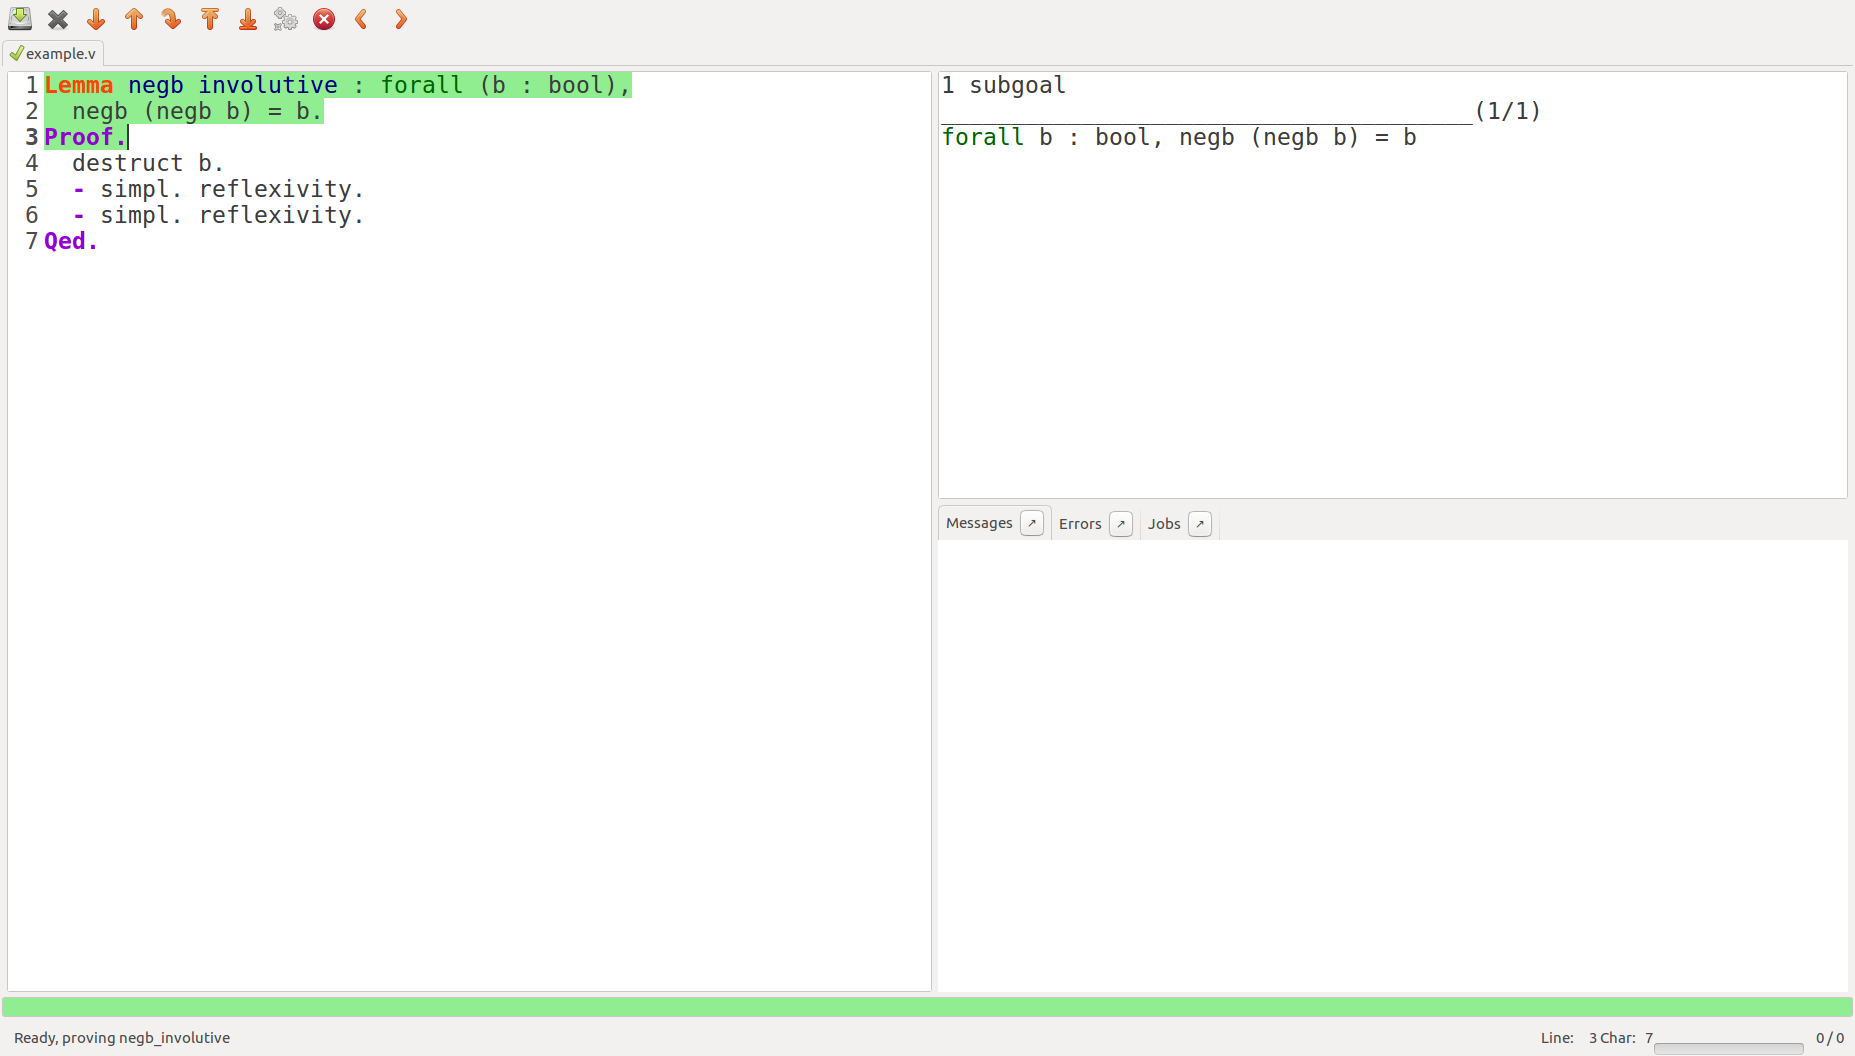
\includegraphics[width=\textwidth]{images/coqide.png}
	\end{center}
\end{figure}

The keywords \coqdoctac{destruct}, \coqdoctac{simpl}, and \coqdoctac{reflexivity} are examples of tactics. A tactic is a command that is used to guide the process of checking some claim we are making. In the context of this proof, the tactic \coqdoctac{destruct} generates two sub-goals, one for each boolean value, which we must prove separately in order to prove the main goal. This strategy is also known as proof by case analysis. The command $-$ is then used to focus on the next generated sub-goal.

The tactic \coqdoctac{simpl} is often used in situations where we want to evaluate a compound expression, eventually reducing it to a simplified, easier-to-understand term. It facilitates our decisions in a proof development by resolving all the computations that can be done in a given state of the goal. Additionally, the tactic \coqdoctac{reflexivity} finishes a proof by showing that both sides of an equation contain identical values.

\begin{longtable}{| S | P |}
	\caption{Proof of lemma negb\_involutive}\\
	\hline
	\coqpsvstephdr & \coqpsvsithdr\\
	\hline
	\endfirsthead

	\caption{Proof of negb\_involutive continued}\\
	\hline
	\coqpsvstephdr & \coqpsvsithdr\\
	\hline
	\endhead

	\multicolumn{2}{r}{Continuing proof of Lemma negb\_involutive on the next page}\\
	\endfoot
	\hline
	\multicolumn{2}{r}{End of proof of Lemma negb\_involutive}\\
	\endlastfoot

	\multirow{2}{*}{$Proof.$} & \fracrule\linebreak
	$forall $ $ b $ $ : $ $ bool, $ $ negb $ $ (negb $ $ b) $ $ = $ $ b$\\

	\hline
	\multirow{4}{*}{$destruct $ $ b.$} & \fracrule\linebreak
	$negb $ $ (negb $ $ true) $ $ = $ $ true$\\
	\cline{2-2}
	& \fracrule\linebreak
	$negb $ $ (negb $ $ false) $ $ = $ $ false$\\

	\hline
	\multirow{2}{*}{$-_{1/2}$} & \fracrule\linebreak
	$negb $ $ (negb $ $ true) $ $ = $ $ true$\\

	\hline
	\multirow{2}{*}{$simpl.$} & \fracrule\linebreak
	$true $ $ = $ $ true$\\

	\hline
	$reflexivity.$ & $-_{1/2}$ completed \\
	\hline
	\multirow{2}{*}{$-_{2/2}$} & \fracrule\linebreak
	$negb $ $ (negb $ $ false) $ $ = $ $ false$\\

	\hline
	\multirow{2}{*}{$simpl.$} & \fracrule\linebreak
	$false $ $ = $ $ false$\\

	\hline
	$reflexivity.$ & $-_{2/2}$ completed, proof completed by Qed \label{Proofs:coq-example:Lemma:negb-involutive} \\
	\hline
\end{longtable}

Once we proved this lemma, it is now available to be used inside other proofs such as the theorem we have stated before. In what follows, we show its proof script.

\begin{coqdoccode}
	\coqdocnoindent
	\coqdockw{Theorem} \coqdocvar{evenb\_S} : \coqdockw{\ensuremath{\forall}} \coqdocvar{n} : \coqdocvar{nat},\coqdoceol
	\coqdocindent{1.00em}
	\coqdocvar{evenb} (\coqdocvar{S} \coqdocvar{n}) = \coqdocvar{negb} (\coqdocvar{evenb} \coqdocvar{n}).\coqdoceol
	\coqdocnoindent
	\coqdockw{Proof}.\coqdoceol
	\coqdocindent{1.00em}
	\coqdoctac{intros}. \coqdoctac{induction} \coqdocvar{n}.\coqdoceol
	\coqdocindent{1.00em}
	- \coqdoctac{simpl}. \coqdoctac{reflexivity}.\coqdoceol
	\coqdocindent{1.00em}
	- \coqdoctac{simpl}. \coqdoctac{simpl} \coqdoctac{in} \coqdocvar{IHn}. \coqdoctac{rewrite} \coqdocvar{IHn}.\coqdoceol
	\coqdocindent{2.00em}
	\coqdoctac{rewrite} \coqdocvar{negb\_involutive}. \coqdoctac{reflexivity}.\coqdoceol
	\coqdocnoindent
	\coqdockw{Qed}.\coqdoceol
\end{coqdoccode}

See the step-by-step proof for Theorem \coqdocvar{evenb\_S} in Table \ref{Proofs:coq-example:Theorem:evenb-S}. The quantifier \coqdockw{\ensuremath{\forall}} \coqdocvar{n}:\coqdocvar{nat} indicates that we want to prove this claim considering all natural numbers $ n $. The tactic \coqdoctac{intros} performs universal instantiation, rewriting the claim considering an arbitrary natural number $ n $, which is declared in the proof context (all definitions above the proof horizontal bar).

This example demonstrates a proof by induction over natural numbers that is made possible in Coq by the \coqdoctac{induction} tactic. Following this principle, to show that a proposition holds for all natural numbers $ n $ we must prove: the base case ($ n = 0 $), and then the induction step, which is, for any number $ n $, if the proposition holds for $ n $, then so it does for $ S \ n $.

The tactic \coqdoctac{rewrite} tells Coq to perform a replacement in the goal, which can be based on an assumption (hypothesis) from the proof context or on a completely separate proof such as the Lemma \coqdocvar{negb\_involutive}.


\begin{longtable}{| S | P |}
	\caption{Proof of theorem evenb\_S}\\
	\hline
	\coqpsvstephdr & \coqpsvsithdr\\
	\hline
	\endfirsthead

	\caption{Proof of Theorem evenb\_S continued}\\
	\hline
	\coqpsvstephdr & \coqpsvsithdr\\
	\hline
	\endhead

	\multicolumn{2}{r}{Continuing proof of Theorem evenb\_S on the next page}\\
	\endfoot
	\hline
	\multicolumn{2}{r}{End of proof of Theorem evenb\_S}\\
	\endlastfoot

	\multirow{2}{*}{$Proof.$} & \fracrule\linebreak
	$forall $ $ n $ $ : $ $ nat, $ $ evenb $ $ (S $ $ n) $ $ = $ $ negb $ $ (evenb $ $ n)$\\

	\hline
	\multirow{3}{*}{$intros.$} & $n$$ $ $ : $ $ nat$\linebreak
	\fracrule\linebreak
	$evenb $ $ (S $ $ n) $ $ = $ $ negb $ $ (evenb $ $ n)$\\

	\hline
	\multirow{7}{*}{$induction $ $ n.$} & \fracrule\linebreak
	$evenb $ $ 1 $ $ = $ $ negb $ $ (evenb $ $ 0)$\\
	\cline{2-2}
	& $n$$ $ $ : $ $ nat$\linebreak
	$IHn$$ $ $ : $ $ evenb $ $ (S $ $ n) $ $ = $ $ negb $ $ (evenb $ $ n)$\linebreak
	\fracrule\linebreak
	$evenb $ $ (S $ $ (S $ $ n)) $ $ = $ $ negb $ $ (evenb $ $ (S $ $ n))$\\

	\hline
	\multirow{2}{*}{$-_{1/2}$} & \fracrule\linebreak
	$evenb $ $ 1 $ $ = $ $ negb $ $ (evenb $ $ 0)$\\

	\hline
	\multirow{2}{*}{$simpl.$} & \fracrule\linebreak
	$false $ $ = $ $ false$\\

	\hline
	$reflexivity.$ & $-_{1/2}$ completed \\
	\hline
	\multirow{5}{*}{$-_{2/2}$} & $n$$ $ $ : $ $ nat$\linebreak
	$IHn$$ $ $ : $ $ evenb $ $ (S $ $ n) $ $ = $ $ negb $ $ (evenb $ $ n)$\linebreak
	\fracrule\linebreak
	$evenb $ $ (S $ $ (S $ $ n)) $ $ = $ $ negb $ $ (evenb $ $ (S $ $ n))$\\

	\hline
	\multirow{6}{*}{$simpl.$} & $n$$ $ $ : $ $ nat$\linebreak
	$IHn$$ $ $ : $ $ evenb $ $ (S $ $ n) $ $ = $ $ negb $ $ (evenb $ $ n)$\linebreak
	\fracrule\linebreak
	$evenb $ $ n $ $ = $ $ negb $ $ match $ $ n $ $ with
	$ $  $ $  $ $  $ $  $ $  $ $  $ $  $ $  $ $  $ $  $ $  $ $  $ $  $ $  $ $ | $ $ 0 $ $ ={>} $ $ false
	$ $  $ $  $ $  $ $  $ $  $ $  $ $  $ $  $ $  $ $  $ $  $ $  $ $  $ $  $ $ | $ $ S $ $ n{\textquotesingle} $ $ ={>} $ $ evenb $ $ n{\textquotesingle}
	$ $  $ $  $ $  $ $  $ $  $ $  $ $  $ $  $ $  $ $  $ $  $ $  $ $  $ $  $ $ end$\\

	\hline
	\multirow{8}{*}{$simpl $ $ in $ $ IHn.$} & $n$$ $ $ : $ $ nat$\linebreak
	$IHn$$ $ $ : $ $ match $ $ n $ $ with
	$ $  $ $  $ $ | $ $ 0 $ $ ={>} $ $ false
	$ $  $ $  $ $ | $ $ S $ $ n{\textquotesingle} $ $ ={>} $ $ evenb $ $ n{\textquotesingle}
	$ $  $ $  $ $ end $ $ = $ $ negb $ $ (evenb $ $ n)$\linebreak
	\fracrule\linebreak
	$evenb $ $ n $ $ = $ $ negb $ $ match $ $ n $ $ with
	$ $  $ $  $ $  $ $  $ $  $ $  $ $  $ $  $ $  $ $  $ $  $ $  $ $  $ $  $ $ | $ $ 0 $ $ ={>} $ $ false
	$ $  $ $  $ $  $ $  $ $  $ $  $ $  $ $  $ $  $ $  $ $  $ $  $ $  $ $  $ $ | $ $ S $ $ n{\textquotesingle} $ $ ={>} $ $ evenb $ $ n{\textquotesingle}
	$ $  $ $  $ $  $ $  $ $  $ $  $ $  $ $  $ $  $ $  $ $  $ $  $ $  $ $  $ $ end$\\

	\hline
	\multirow{7}{*}{$rewrite $ $ IHn.$} & $n$$ $ $ : $ $ nat$\linebreak
	$IHn$$ $ $ : $ $ match $ $ n $ $ with
	$ $  $ $  $ $ | $ $ 0 $ $ ={>} $ $ false
	$ $  $ $  $ $ | $ $ S $ $ n{\textquotesingle} $ $ ={>} $ $ evenb $ $ n{\textquotesingle}
	$ $  $ $  $ $ end $ $ = $ $ negb $ $ (evenb $ $ n)$\linebreak
	\fracrule\linebreak
	$evenb $ $ n $ $ = $ $ negb $ $ (negb $ $ (evenb $ $ n))$\\

	\hline
	\multirow{6}{*}{\shortstack[l]{$rewrite $\\ $ negb{\char`\_}involutive.$}} & $n$$ $ $ : $ $ nat$\linebreak
	$IHn$$ $ $ : $ $ match $ $ n $ $ with
	$ $  $ $  $ $ | $ $ 0 $ $ ={>} $ $ false
	$ $  $ $  $ $ | $ $ S $ $ n{\textquotesingle} $ $ ={>} $ $ evenb $ $ n{\textquotesingle}
	$ $  $ $  $ $ end $ $ = $ $ negb $ $ (evenb $ $ n)$\linebreak
	\fracrule\linebreak
	$evenb $ $ n $ $ = $ $ evenb $ $ n$\\

	\hline
	$reflexivity.$ & $-_{2/2}$ completed, proof completed by Qed \label{Proofs:coq-example:Theorem:evenb-S} \\
	\hline
\end{longtable}

To illustrate other tactics, consider another theorem on natural numbers: for all $ n $, if $ n $ is even, then the predecessor of the predecessor of $ n $ is also even. This theorem can be proved in Coq as follows. Note that here we are referring to the inductive definition of evenness (\emph{ev}).

\begin{coqdoccode}
	\coqdocnoindent
	\coqdockw{Theorem} \coqdocvar{ev\_minus2} : \coqdockw{\ensuremath{\forall}} \coqdocvar{n}:\coqdocvar{nat},\coqdoceol
	\coqdocindent{1.00em}
	\coqdocvar{ev} \coqdocvar{n} \ensuremath{\rightarrow} \coqdocvar{ev} (\coqdocvar{pred} (\coqdocvar{pred} \coqdocvar{n})).\coqdoceol
	\coqdocnoindent
	\coqdockw{Proof}.\coqdoceol
	\coqdocindent{1.00em}
	\coqdoctac{intros}.\coqdoceol
	\coqdocindent{1.00em}
	\coqdoctac{destruct} \coqdocvar{H}.\coqdoceol
	\coqdocindent{1.00em}
	- \coqdoctac{simpl}. \coqdoctac{apply} \coqdocvar{ev\_0}.\coqdoceol
	\coqdocindent{1.00em}
	- \coqdoctac{simpl}. \coqdoctac{apply} \coqdocvar{H}.\coqdoceol
	\coqdocnoindent
	\coqdockw{Qed}.\coqdoceol
\end{coqdoccode}

See the proof for Theorem \coqdocvar{ev\_minus2} in Table \ref{Proofs:coq-example:Theorem:ev-minus2}. In this proof, besides performing universal instantiation, the tactic \coqdoctac{intros} moves the implication antecedent to the proof context as a hypothesis. One needs to prove the implication consequent assuming that its antecedent is true; otherwise, the claim would be trivially true since, from contradiction, anything follows (the \emph{Ex falso quodlibet} principle).

As we have discussed before, the tactic \coqdoctac{destruct} performs proof by case analysis. In this example, it is responsible for generating, from the hypothesis, two sub-goals based on the inductive definition of evenness we have provided: one where $ n = 0 $ and another where $ n = S \ (S \ n) $. Once again, we must prove them separately so Coq accepts the theorem.

\begin{longtable}{| S | P |}
	\caption{Proof of Theorem ev\_minus2}\\
	\hline
	\coqpsvstephdr & \coqpsvsithdr\\
	\hline
	\endfirsthead

	\caption{Proof of Theorem ev\_minus2 continued}\\
	\hline
	\coqpsvstephdr & \coqpsvsithdr\\
	\hline
	\endhead

	\multicolumn{2}{r}{Continuing proof of Theorem ev\_minus2 on the next page}\\
	\endfoot
	\hline
	\multicolumn{2}{r}{End of proof of Theorem ev\_minus2}\\
	\endlastfoot

	\multirow{2}{*}{$Proof.$} & \fracrule\linebreak
	$forall $ $ n $ $ : $ $ nat, $ $ ev $ $ n $ $ -{>} $ $ ev $ $ (pred $ $ (pred $ $ n))$\\

	\hline
	\multirow{4}{*}{$intros.$} & $n$$ $ $ : $ $ nat$\linebreak
	$H$$ $ $ : $ $ ev $ $ n$\linebreak
	\fracrule\linebreak
	$ev $ $ (pred $ $ (pred $ $ n))$\\

	\hline
	\multirow{6}{*}{$destruct $ $ H.$} & \fracrule\linebreak
	$ev $ $ (pred $ $ (pred $ $ 0))$\\
	\cline{2-2}
	& $n$$ $ $ : $ $ nat$\linebreak
	$H$$ $ $ : $ $ ev $ $ n$\linebreak
	\fracrule\linebreak
	$ev $ $ (pred $ $ (pred $ $ (S $ $ (S $ $ n))))$\\

	\hline
	\multirow{2}{*}{$-_{1/2}$} & \fracrule\linebreak
	$ev $ $ (pred $ $ (pred $ $ 0))$\\

	\hline
	\multirow{2}{*}{$simpl.$} & \fracrule\linebreak
	$ev $ $ 0$\\

	\hline
	$apply $ $ ev{\char`\_}0.$ & $-_{1/2}$ completed \\
	\hline
	\multirow{4}{*}{$-_{2/2}$} & $n$$ $ $ : $ $ nat$\linebreak
	$H$$ $ $ : $ $ ev $ $ n$\linebreak
	\fracrule\linebreak
	$ev $ $ (pred $ $ (pred $ $ (S $ $ (S $ $ n))))$\\

	\hline
	\multirow{4}{*}{$simpl.$} & $n$$ $ $ : $ $ nat$\linebreak
	$H$$ $ $ : $ $ ev $ $ n$\linebreak
	\fracrule\linebreak
	$ev $ $ n$\\

	\hline
	$apply $ $ H.$ & $-_{2/2}$ completed, proof completed by Qed \label{Proofs:coq-example:Theorem:ev-minus2} \\
	\hline
\end{longtable}

We then proceed to use the tactic \coqdoctac{apply}, passing the term we find useful for proving each sub-goal as argument. In the first branch, where our goal is to prove $ ev \ 0 $, we apply the first rule of our inductive definition, $ ev\_0 $, which concludes this sub-proof, since it provides evidence that $ ev \ 0 $ is true. In the second branch, after simplification, we have $ ev \ n $ as goal, which is already an assumption of ours (introduced to the proof context by the command \coqdoctac{intros}). In this situation, the tactic \coqdoctac{apply} also concludes the second sub-proof, thus proving the entire statement (theorem \coqdocvar{ev\_minus2}).

There are many other tactics and variations that can be used when proving a proposition. Apart from the ones we have already discussed in this section, other commonly used tactic commands are \coqdoctac{unfold}, \coqdoctac{inversion}, and \coqdoctac{contradiction}. Further explanation on these tactics will be provided as needed.

% ---
\subsection{The tactics language}
% ---

Ltac is the tactics language for Coq. It provides the user with a high-level ``toolbox''  for tactics creation, allowing one to build complex tactics by combining existing ones with constructs such as conditionals, looping, backtracking, and error catching.

Imagine we want to prove that the number 4 does not appear in the list of consecutive natural numbers ranging from 0 to 3. By using the keyword \coqdockw{Example}, we can assert this statement in Coq and develop our proof. See the proof script in what follows.

\begin{coqdoccode}
	\coqdocnoindent
	\coqdockw{Example} \coqdocvar{elem\_not\_in\_list} : \ensuremath{\lnot} (\coqdocvar{In} 4 [0 ; 1 ; 2 ; 3]).\coqdoceol
	\coqdocnoindent
	\coqdockw{Proof}.\coqdoceol
	\coqdocindent{1.00em}
	\coqdoctac{unfold} \coqdocvar{not}. \coqdoctac{simpl}. \coqdoctac{intros}.\coqdoceol
	\coqdocindent{1.00em}
	\coqdoctac{destruct} \coqdocvar{H}.\coqdoceol
	\coqdocindent{1.00em}
	- \coqdoctac{inversion} \coqdocvar{H}.\coqdoceol
	\coqdocindent{1.00em}
	- \coqdoctac{destruct} \coqdocvar{H}.\coqdoceol
	\coqdocindent{2.00em}
	\ensuremath{\times} \coqdoctac{inversion} \coqdocvar{H}.\coqdoceol
	\coqdocindent{2.00em}
	\ensuremath{\times} \coqdoctac{destruct} \coqdocvar{H}.\coqdoceol
	\coqdocindent{3.00em}
	+ \coqdoctac{inversion} \coqdocvar{H}.\coqdoceol
	\coqdocindent{3.00em}
	+ \coqdoctac{destruct} \coqdocvar{H}.\coqdoceol
	\coqdocindent{4.00em}
	\{ \coqdoctac{inversion} \coqdocvar{H}. \}\coqdoceol
	\coqdocindent{4.00em}
	\{ \coqdoctac{contradiction}. \}\coqdoceol
	\coqdocnoindent
	\coqdockw{Qed}.\coqdoceol
\end{coqdoccode}

The first tactic unfolds the definition of \ensuremath{\lnot} (not) in the goal, replacing our initial statement by \coqdocvar{In} 4 [0 ; 1 ; 2 ; 3] \ensuremath{\rightarrow} \coqdocvar{False}. In Coq, the logical negation of $P$ is defined as follows: $P$ \ensuremath{\rightarrow} \coqdocvar{False}. Therefore, if $P$ is true, the obtained proposition is false; if $P$ is false, the obtained proposition is true, as expected.

The second tactic reduces the new goal by computing the function \coqdocvar{In}, which leaves us with the disjunctions $ 0 = 4 \lor 1 = 4 \lor 2 = 4 \lor 3 = 4 \lor \coqdocvar{False} $ in the antecedent of the implication. Then, the tactic \coqdoctac{intros} moves this antecedent to the proof context, introducing a new hypothesis \coqdocvar{H} and leaving the literal \coqdocvar{False} as the proof goal.

From this point on, the proof has the following pattern: we perform a destruction followed by an inversion of the hypothesis until we can end the proof by contradiction. The recurrence of the tactic \coqdoctac{destruct} lets us focus in one equality from the disjunction at a time: first the hypothesis becomes $ 0 = 4 $, then $ 1 = 4 $ and so on. The tactic \coqdoctac{inversion} finishes each sub-proof created by the previous command by deriving all the necessary conditions that should hold for the assumption to be proved. In this case, since none of these equalities is true, there is no condition that satisfies the proposition, thus proving our goal. The tactic \coqdoctac{contradiction} finishes the proof by searching for a \emph{contradiction} in the proof context. We also note the use of $-$, $\times$, $+$ and $\{ \}$ to focus on nested sub-goals.

Since this pattern in the sequence of tactics is now exposed, we can define a tactic macro for proving propositions of the format ``not in'' using the keyword \coqdockw{Ltac}:

\begin{coqdoccode}
	\coqdocnoindent
	\coqdockw{Ltac} \coqdocvar{solve\_not\_in} := \coqdoctac{unfold} \coqdocvar{not};\coqdoceol
	\coqdocindent{1.00em}
	\coqdockw{let} \coqdocvar{H} := \coqdoctac{fresh} ``H'' \coqdoctac{in} (\coqdoceol
	\coqdocindent{2.00em}
	\coqdoctac{intros} \coqdocvar{H}; \coqdoctac{repeat} (\coqdoctac{contradiction} + (\coqdoctac{destruct} \coqdocvar{H}; [> \coqdoctac{inversion} \coqdocvar{H} \ensuremath{|} ]))\coqdoceol
	\coqdocindent{1.00em}
	).\coqdoceol
\end{coqdoccode}

The new tactic \coqdocvar{solve\_not\_in} works by first unfolding the function \coqdocvar{not} (the propositional function that represents the logical not in Coq), therefore deriving an implication. Then it moves the implication antecedent to the proof context. Finally, it repeats the following steps until the proof is finished: try to finish the proof by searching for a \emph{contradiction} in the assumptions (such as a false hypothesis); if it fails, \emph{destruct} the hypothesis and apply \emph{inversion} to it in order to prove the first sub-goal yielded by the previous tactic. With this new user-defined tactic, the previous example can now be provided as follows.

\begin{coqdoccode}
	\coqdocemptyline
	\coqdocnoindent
	\coqdockw{Example} \coqdocvar{elem\_not\_in\_list'} : \ensuremath{\lnot} (\coqdocvar{In} 4 [0 ; 1 ; 2 ; 3]).\coqdoceol
	\coqdocnoindent
	\coqdockw{Proof}. \coqdocvar{solve\_not\_in}. \coqdockw{Qed}.\coqdoceol
\end{coqdoccode}

As one can see, with no further user intervention besides invoking the appropriate tactic. Furthermore, this proof script would work for lists of arbitrary size. Therefore, we say that \coqdocvar{solve\_not\_in} describes a decision procedure for proving that some element is not a member of a given list.

% ---
\section{QuickChick}
\label{section:quickchick}
% ---

QuickChick is a set of tools and techniques for combining randomised property-based testing with formal specifications and proofs in the Coq ecosystem. It is the Coq equivalent of Haskell's QuickCheck tool.

There are four basic elements in property-based random testing: an \emph{executable property}, \emph{generators} of random inputs to the property, \emph{printers} for converting data structures like numbers to strings when reporting counterexamples, and \emph{shrinkers}, which are used to search for minimal counterexamples when errors occur.

Consider the following example extracted from \citeonline{Lampropoulos:SF4}. The function \emph{remove} takes a natural number $ x $ and a list of natural numbers $ l $ and removes (the first occurence of) $ x $ from the list.

\begin{coqdoccode}
	\coqdocnoindent
	\coqdockw{Fixpoint} \coqdocvar{remove} (\coqdocvar{x} : \coqdocvar{nat}) (\coqdocvar{l} : \coqdocvar{list} \coqdocvar{nat}) : \coqdocvar{list} \coqdocvar{nat} :=\coqdoceol
	\coqdocindent{1.00em}
	\coqdockw{match} \coqdocvar{l} \coqdockw{with}\coqdoceol
	\coqdocindent{2.00em}
	\ensuremath{|} []   \ensuremath{\Rightarrow} []\coqdoceol
	\coqdocindent{2.00em}
	\ensuremath{|} \coqdocvar{h}::\coqdocvar{t} \ensuremath{\Rightarrow} \coqdockw{if} \coqdocvar{h} =? \coqdocvar{x} \coqdockw{then} \coqdocvar{t} \coqdockw{else} \coqdocvar{h} :: \coqdocvar{remove} \coqdocvar{x} \coqdocvar{t}\coqdoceol
	\coqdocindent{1.00em}
	\coqdockw{end}.\coqdoceol
\end{coqdoccode}

We can write assertions that represent our expectations regarding this function. One possible specification for \emph{remove} could be the following property:

\begin{coqdoccode}
	\coqdocnoindent
	\coqdockw{Conjecture} \coqdocvar{removeP} : \coqdockw{\ensuremath{\forall}} \coqdocvar{x} \coqdocvar{l},  \ensuremath{\lnot} (\coqdocvar{In} \coqdocvar{x} (\coqdocvar{remove} \coqdocvar{x} \coqdocvar{l})).\coqdoceol
\end{coqdoccode}

The keyword \coqdockw{Conjecture} treats our property \coqdocvar{removeP} as an axiom. This proposition claims that $ x $ never occurs in the result of $ \mathit{remove} \ x \ l $ for any $ x $ and $ l $. Such statement turns out to be false, as we would discover if we were to try to prove it. A different — perhaps much more efficient — way to discover the discrepancy between the definition and specification is to test it using QuickChick.

\begin{coqdoccode}
	\coqdocnoindent
	\coqdocvar{QuickChick} \coqdocvar{removeP}.\coqdoceol
\end{coqdoccode}

The \coqdocvar{QuickChick} command takes an executable property and attempts to falsify it by running it on many randomly generated inputs, resulting in an output as follows.

\begin{tabbing}
	\emph{0} \\
	\emph{[0, 0]} \\
	\emph{Failed! After 17 tests and 12 shrinks}
\end{tabbing}

This means that, if we run \emph{remove} with $ x $ being 0 and $ l $ being the two-element list containing two zeros, then the property \coqdocvar{removeP} fails. With this example in hand, we can see that the \emph{then} branch of \emph{remove} fails to make a recursive call, which means that only the first occurrence of $ x $ will be removed from the list. The last line of the output records that 17 tests were necessary to identify some fault-inducing input and 12 shrinks to reduce it to a minimal counterexample. 	It is important to emphasise that QuickChick is a testing-based tool and, thus, if it does not find a counterexample for a given property, it does not necessarily mean that the property is correct indeed.

